
% Template for Elsevier CRC journal article
% version 1.1 dated 16 March 2010

% This file (c) 2010 Elsevier Ltd.  Modifications may be freely made,
% provided the edited file is saved under a different name

% This file contains modifications for Procedia Computer Science
% but may easily be adapted to other journals

% Changes since version 1.0
% - elsarticle class option changed from 1p to 3p (to better reflect CRC layout)

%-----------------------------------------------------------------------------------

%% This template uses the elsarticle.cls document class and the extension package ecrc.sty
%% For full documentation on usage of elsarticle.cls, consult the documentation "elsdoc.pdf"
%% Further resources available at http://www.elsevier.com/latex

%-----------------------------------------------------------------------------------

%%%%%%%%%%%%%%%%%%%%%%%%%%%%%%%%%%%%%%%%%%%%%%
%%%%%%%%%%%%%%%%%%%%%%%%%%%%%%%%%%%%%%%%%%%%%%
%%                                          %%
%% Important note on usage                  %%
%% -----------------------                  %%
%% This file must be compiled with PDFLaTeX %%
%% Using standard LaTeX will not work!      %%
%%                                          %%
%%%%%%%%%%%%%%%%%%%%%%%%%%%%%%%%%%%%%%%%%%%%%%
%%%%%%%%%%%%%%%%%%%%%%%%%%%%%%%%%%%%%%%%%%%%%%

%% The '3p' and 'times' class options of elsarticle are used for Elsevier CRC
\documentclass[3p,times]{elsarticle}

%% The `ecrc' package must be called to make the CRC functionality available
\usepackage{ecrc}

%% The ecrc package defines commands needed for running heads and logos.
%% For running heads, you can set the journal name, the volume, the starting page and the authors

%% set the volume if you know. Otherwise `00'
\volume{00}

%% set the starting page if not 1
\firstpage{1}

%% Give the name of the journal
\journalname{NUCLEAR INSTRUMENTS AND METHODS
IN PHYSICS RESEARCH}

%% Give the author list to appear in the running head
%% Example \runauth{C.V. Radhakrishnan et al.}
\runauth{D. E. Holland et al.}

%% The choice of journal logo is determined by the \jid and \jnltitlelogo commands.
%% A user-supplied logo with the name <\jid>logo.pdf will be inserted if present.
%% e.g. if \jid{yspmi} the system will look for a file yspmilogo.pdf
%% Otherwise the content of \jnltitlelogo will be set between horizontal lines as a default logo

%% Give the abbreviation of the Journal.
\jid{NIM:A}

%% Give a short journal name for the dummy logo (if needed)
\jnltitlelogo{NIM:A}

%% Hereafter the template follows `elsarticle'.
%% For more details see the existing template files elsarticle-template-harv.tex and elsarticle-template-num.tex.

%% Elsevier CRC generally uses a numbered reference style
%% For this, the conventions of elsarticle-template-num.tex should be followed (included below)
%% If using BibTeX, use the style file elsarticle-num.bst

%% End of ecrc-specific commands
%%%%%%%%%%%%%%%%%%%%%%%%%%%%%%%%%%%%%%%%%%%%%%%%%%%%%%%%%%%%%%%%%%%%%%%%%%

%% The amssymb package provides various useful mathematical symbols
\usepackage{amssymb}
%% The amsthm package provides extended theorem environments
\usepackage{amsthm}
\usepackage{amsmath}

%% The lineno packages adds line numbers. Start line numbering with
%% \begin{linenumbers}, end it with \end{linenumbers}. Or switch it on
%% for the whole article with \linenumbers after \end{frontmatter}.
\usepackage{lineno}
\modulolinenumbers[5]

%% natbib.sty is loaded by default. However, natbib options can be
%% provided with \biboptions{...} command. Following options are
%% valid:

%%   round  -  round parentheses are used (default)
%%   square -  square brackets are used   [option]
%%   curly  -  curly braces are used      {option}
%%   angle  -  angle brackets are used    <option>
%%   semicolon  -  multiple citations separated by semi-colon
%%   colon  - same as semicolon, an earlier confusion
%%   comma  -  separated by comma
%%   numbers-  selects numerical citations
%%   super  -  numerical citations as superscripts
%%   sort   -  sorts multiple citations according to order in ref. list
%%   sort&compress   -  like sort, but also compresses numerical citations
%%   compress - compresses without sorting
%%
%% \biboptions{comma,round}

% \biboptions{}

% if you have landscape tables
\usepackage[figuresright]{rotating}

% put your own definitions here:
%   \newcommand{\cZ}{\cal{Z}}
%   \newtheorem{def}{Definition}[section]
%   ...

% add words to TeX's hyphenation exception list
%\hyphenation{author another created financial paper re-commend-ed Post-Script}

% declarations for front matter

\begin{document}

\begin{frontmatter}

%% Title, authors and addresses

%% use the tnoteref command within \title for footnotes;
%% use the tnotetext command for the associated footnote;
%% use the fnref command within \author or \address for footnotes;
%% use the fntext command for the associated footnote;
%% use the corref command within \author for corresponding author footnotes;
%% use the cortext command for the associated footnote;
%% use the ead command for the email address,
%% and the form \ead[url] for the home page:
%%
%% \title{Title\tnoteref{label1}}
%% \tnotetext[label1]{}
%% \author{Name\corref{cor1}\fnref{label2}}
%% \ead{email address}
%% \ead[url]{home page}
%% \fntext[label2]{}
%% \cortext[cor1]{}
%% \address{Address\fnref{label3}}
%% \fntext[label3]{}

\dochead{}
%% Use \dochead if there is an article header, e.g. \dochead{Short communication}

\title{Rotating Scatter Mask Optimization for Gamma Source Direction Identification}

%% use optional labels to link authors explicitly to addresses:
%% \author[label1,label2]{<author name>}
%% \address[label1]{<address>}
%% \address[label2]{<address>}

\author[d1]{Darren E. Holland}
\author[d2]{James E. Bevins}
\author[d2]{Larry W. Burggraf\ }
\author[d2]{Buckley E. O'Day}

\address[d1]{dholland@cedarville.edu\\
  Department of Mechanical Engineering\\
	Cedarville University \\
	Cedarville, OH\\}
	
\address[d2]{Department of Engineering Physics\\
	Air Force Institute of Technology \\
	Wright-Patterson AFB, OH\\}

\begin{abstract}
Rotating scattering masks have shown promise as an inexpensive, lightweight method with a large field-of-view for identifying the direction of a gamma emitting source
or sources.  However, further examination of the current rotating scattering mask design shows that changing the geometry may improve the identification by reducing or eliminating degenerate solutions and lower required count times.  
These changes should produce more linearly independent characteristics for the mask, resulting in a decrease in the mis-identification probability.  
Three approaches are introduced to generate alternative mask geometries.
The eigenvector method uses a spring-mass system to create a geometry basis.  The binary approach uses ones and zeros to represent the geometry with many possible
combinations allowing for additional design flexibility.  
Finally, a Hadamard matrix is modified to examine a decoupled geometric solution.   
Four criteria are proposed for evaluating these methodologies.
An analysis of the resulting detector response matrices demonstrates that these methodologies produced 
superior identification characteristics than the original design.  The eigenvector approach produces the least linearly dependent results, but exhibits a decrease
in average efficiency.  The binary results are more linearly dependent than the eigenvector approach, but this design achieves a higher average efficiency than than original.  
The Hadamard-based method produced a lower maximum, but a higher average linear dependence than the original design.
Further possible design enhancements are discussed.
\end{abstract}

\begin{keyword}
%% keywords here, in the form: keyword \sep keyword
RSM \sep geometry optimization \sep Hadamard \sep source direction
%% MSC codes here, in the form: \MSC code \sep code
%% or \MSC[2008] code \sep code (2000 is the default)

\end{keyword}

\end{frontmatter}

%%
%% Start line numbering here if you want
%%
\linenumbers

%% main text
\section{Introduction}
\label{intro}
Identifying a gamma source's direction is important in a variety of applications such as providing security, treaty compliance verification, and locating orphan sources.  
Three general categories exist for gamma source direction identification; count-based systems, collimator and coded aperture systems, and Compton cameras.
In count-based systems, a source's direction is determined by the relative change in the count number as the detector changes positions.  This method can 
be inefficient and increase the user's exposure as they search for the source.  Collimator and coded aperture systems 
use intervening material or a mask to create a unique detection pattern, which can be
used to identify the source's direction.  However, the intervening material reduces
the detector's field-of-view (FOV) \cite{Vetter06}, which increases the time required to survey surrounding areas.  For higher gamma energy levels, the system's weight 
and portability can become problematic as shown by the 32,000 lb SuperMISTI system \cite{Hutcheson14} and 2700 lb Large-Area Imager \cite{Ziock06}.  
These systems are mounted on mobile platforms in order to image
the area of interest.  Compton cameras offer up to a 4$\pi$ FOV 
\cite{Wahl11} and can distinguish between background and source radiation \cite{Vetter06, Phillips95}.  However,
these systems require Compton events and ignore the full-energy-peak (FEP) 
direction information.

A novel approach, similar in concept to the coded aperture system, exists that eliminates many of the alternative's limitations.
This system utilizes a mask placed over a single position-insensitive detector \cite{FitzGerald2015}.  
The system records energy spectra as a function of the geometrically varying mask, which is accomplished through a set, constant mask rotation. 
The obtained position dependent spectra, referred to as detector response curves (DRCs), depend on the source position and can be used to identify the source direction.  FitzGerald's mask geometry results in some DRCs that are nearly identical, which can lead to mis-identification of the source direction.  
This work seeks to reduce the DRCs' linear dependence by optimizing the mask's geometry.

The rotating scatter mask (RSM) concept offers many benefits over other gamma source position identification detectors.  
Specifically, it ``provides a nearly 4$\pi$ field-of-view, operates for a broad range of gamma energies, and has a relatively simple design \cite{Logan2017}." 
This system uses a spherical reference system, where $\theta$ is the azimuthal and $\phi$ the polar angle.  
The mask works by attenuating and scattering the incoming particles in order to produce unique detector response curves \cite{Logan2017}.  
To obtain the measurements for the position identification, the mask starts at an initial $\theta$ and $\phi$ position.
It then rotates in $\theta$ around the detector with the signal recorded at each discrete $\theta$ position.  
The measured DRC is generated by summing the counts over a desired energy range for each $\theta$ position in one complete mask rotation.  
Comparing this curve with each possible DRC, which are known through experimentation or simulation using a mean square error, least squares, or maximum likelihood estimate approach provides an identified initial source direction.

FitzGerald introduced the RSM shown in Fig.~\ref{fig:RSM} that has a 14 inch diameter and surrounds a 3 x 3 inch cylindrical NaI scintillating detector \cite{FitzGerald2015}. 
His original MCNP model contained 31 elements or one element every $11.6^\circ$.  
In order to increase the accuracy of the geometric representations,  the model's angular resolution was later increased to every degree.  

\begin{figure}[ht!]
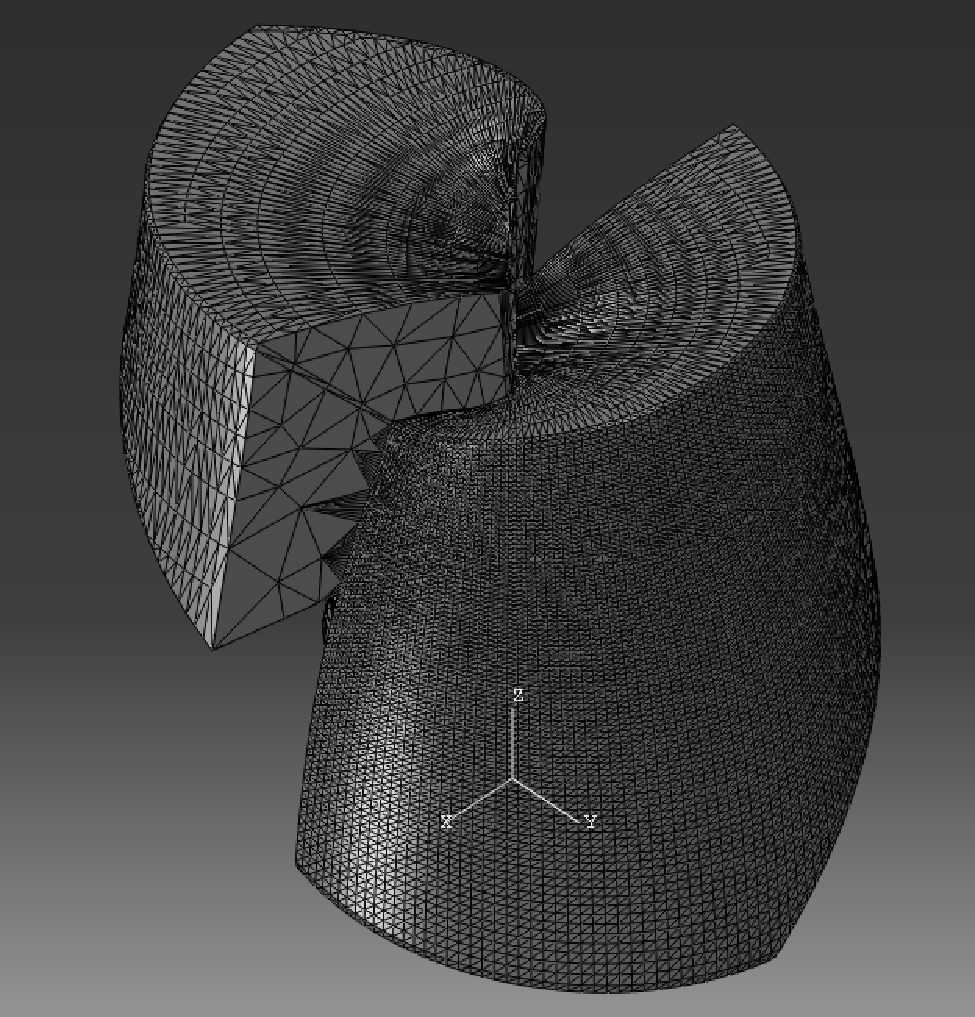
\includegraphics[width={3.0in}]{../figs/P2AtIso.pdf}
\centering
\caption{Isometric view of the unstructured mesh used to model the Fitzgerald RSM in MCNP.}
\label{fig:RSM}
\end{figure}

FitzGerald's design methodology assumes that the detector response is related to the mask geometry.  
Without this assumption, intentional mask design degenerates into random trial and error.
In addition, he proposed three desirable characteristics for the RSM system.  
First, for any given initial source position, there is a unique response curve generated as the mask rotates 360$^\circ$.  
This condition is necessary as a non-unique response would make at least two initial source position DRCs indistinguishable and a unique identification impossible.
The second characteristic requires the mask's average thickness over a 360$^\circ$ rotation to be a constant value for all $\phi$s.  
This criteria prevents higher or lower average responses for different $\phi$ positions. 
This is not necessary to ensure the uniqueness of the DRC; however, DRCs with widely varying average thicknesses may have a lower average count, which makes them more susceptible to measurement noise and increases the time required to obtain an accurate measured response.
The final characteristic is for the solid angle from the detector centroid to be equal for all cells.  
This constraint provides the same spatial resolution in both azimuthal and polar directions.
Not explicitly mentioned by FitzGerald is an assumption that the geometry should be continuous, thereby allowing the DRCs to be discretized as desired.

The remainder of this paper is organized as follows.
Section~\ref{sec:rsm-design} provides an overview of the RSM setup, design assumptions and limitations, design criteria, and the design methodologies used to generate improved RSM designs. 
Section~\ref{sec:results} describes the performance of each of the alternative designs and compares that performance to the Fitzgerald baseline.  
Finally, Section~\ref{sec:conclusions} discusses possible future improvements on the methodologies presented here and key results from the improved RSM designs. 

\section{RSM Design} \label{sec:rsm-design}
Logan et al.\cite{Logan2017} showed statistical agreement between experimental and simulated DRCs using GEANT4 \cite{Agostinelli03} and simulated to simulated DRCs using GEANT4 and MCNP \cite{Goorley13}.
Thus, this work will use MCNP to simulate the experimental DRCs needed for evaluating each RSM design's performance.  
Instead of using only the full energy peak (FEP), the DRC for this work is formed by summing all counts above 200keV to increase the source direction identification's efficiency.  
The 200keV limit was chosen as Logan et al. noted discrepancies for counts below this value due to scatter in the environmental elements not considered in the model \cite{Logan2017}.

Originally, both the analysis of FitzGerald's RSM and the new designs were to be discretized into 10$^\circ$ increments in $\theta$ and 5$^\circ$ in $\phi$.  
However, due to requirements for the Hadamard method, (which is discussed in Section~\ref{sec:decoupling})
the proposed designs are broken into 32 discrete angles in $\theta$ resulting in $\Delta\theta=11.25^\circ$ and $\Delta\phi=5.625^\circ$ for 30 angles in $\phi$.

The RSM design is to be optimized for a $^{137}$Cs point source located 36 inches from the center of the detector, mimicking Logan et. al's setup \cite{Logan2017}.  
To simulate the relative source rotation in MCNP, the mask is stationary, while the source is rotated in spherical coordinates every increment for $\theta$ from 0 to $348.75^\circ$ and for each $\phi$ from 5.625$^\circ$ to $168.75^\circ$.  
The modeled NaI detector includes a 1/8 inch 2024 Aluminum alloy sleeve on which the acrylic RSM is placed. 
The maximum width of the RSM depends on the methodology, but the maximum mask thickness is a constant 7.87 inches (20 cm).  
A sphere of air surrounds the source and detector, and all other environmental factors were ignored.  
To increase the solution convergence rate, particles were emitted within a $27.26^\circ$ half angle cone extending from the source to the detector's center.  
This variance reduction technique assumes that the effect of the few particles that 
scatter in the air outside of the cone, though the mask, and into the detector will have negligible contributions to the simulated DRCs.   
In addition, a 0.095 inch air gap between the mask and aluminum sleeve constrains the mask geometry from impinging on the sleeve and provides a space for grease to be applied between the moving parts.
Finally, due to manufacturing constraints, each mask angle must have a non-zero thickness.

\subsection{Design Assumptions and Limitations}
It is assumed that the detector-mask-source geometry is related to the DRC and that geometry can be reconstructed using the DRC.
Qualitative studies of this correlation showed that, in general, this assumption is valid with two qualifications.  
First, a discontinuous geometry results in a continuous DRC due to correlations with neighboring rotations. 
Second, while the RSM may offer an increase in the total counts, it comes with a limit on the spacial resolution. 
To understand this statement in detail, consider a rectangular prism cell with a given thickness extending from the centroid of the detector (outside of the aluminum sleeve) in a given direction.
Since the cells do not have impenetrable walls, particles from one source position enter cells pointed at other positions.  
In fact, this phenomena is one of the desirable characteristics of FitzGerald's design as an increase in scattered particles can increase the total number of counts seen by the detector thereby increasing the efficiency.  
However, if the cells are too small relative to the source's distance, then neighboring cells may see a response comparable to the cell located between the detector and source.

To best enable source direction identification, a unique set of DRCs must be obtained. 
The complete set of DRCs for all rotations angles forms the design response matrix (DRM).
The primary criterion for the design choice will be the design with the most unique DRM.  
To achieve this goal, the requirements for maintaining a constant spatial resolution in both spherical directions and requiring a continuous geometry are relaxed.  
However, to obtain a more constant response level, a constant average thickness for each $\phi$ angle is maintained.  

For this application, it is desirable that the curve generated at each initial source position be orthogonal - a.k.a. unique - to the others.  
Let this curve be denoted $\mathbf{DRC}_{i,j},$ where $i=0,1,...,n$ is the initial $\theta$ and $j=0,1,...,m$ is the initial $\phi$ index relative to a reference location on the mask.  
Since the mask rotates, the $i^{th}$ DRC will be identical to $\mathbf{DRC}_{g,j}$ shifted by $g-i$ indices.   
A negative number corresponds to a shift to the left and a positive number a shift to the right.  
This property greatly impacts the mask design as any periodic vector with respect to $\theta$ will then result in duplicate $i$ and $g$ DRCs.  
The duplication due to periodicity would fail to meet the design's uniqueness requirements.

\subsection{Modal Assurance Criterion} \label{sec:MAC}
The modal assurance criterion (MAC) is a normalized number that indicates the similarity between two vectors \cite{Allemang03}.
A MAC value of zero indicates the two vectors are orthogonal, while a value of one indicates that they are identical.  

Logan's work established a connection between the measured and the simulated DRCs.
Thus, assuming the measured response can be represented by the simulated spectrum, it is possible to analyze the uniqueness of the design by comparing each DRC with every other possible DRC to find the worst performance.  Eqn.~\ref{eq:mac} defines the MAC number as

\begin{equation}
MAC_{g,h,i,j}=\frac{\left(\mathbf{u}_{g,h}^T\mathbf{v}_{i,j}\right)^2}{\left(\mathbf{u}_{g,h}^T\mathbf{u}_{g,h}\right)\left(\mathbf{v}_{i,j}^T\mathbf{v}_{i,j}\right)},
\label{eq:mac}
\end{equation}

\noindent where $\mathbf{u}_{g,h}$ and $\mathbf{v}_{i,j}$ are the DRCs for the respective initial positions $\left(\theta=g\Delta\theta,\phi=h\Delta\phi\right)$ and
$\left(\theta=i\Delta\theta,\phi=j\Delta\phi\right)$.

Considering all vector shifts, the maximum MAC number, which corresponds to the most similar pair of DRCs is given in Eqn.~\ref{eq:maxmac}.

\begin{equation}
M=max_{g,h,i,j}\left(MAC_{g,h,i,j}\right),
\label{eq:maxmac}
\end{equation}

\noindent where $g\neq i$ and $h\neq j$.  An examination of Eqn.~\ref{eq:maxmac} shows that a bias in vectors $u$ and $v$ will result in a non-zero $M$ value.  
Thus, the DRCs are normalized such that each one is zero mean over $\theta$.  
These normalized DRCs form the reduced DRM or $\bf{DRM_{red}}$. 

\subsection{Design Methodologies} \label{design-methods}
There are two general classes for the geometry creation.  
The first method assumes that both the initial $\theta$ and $\phi$ positions are to be identified.  
The second approach uses a geometric marker, which allows the initial $\theta$ location to be calculated.  
This assumption simplifies the $\theta$ identification and removes the $\theta$ shift effects.  
Both of these classes create a two dimensional matrix, which is mapped as the mask thickness to three dimensional space using spherical coordinates.

\subsubsection{Identifying $\theta$ and $\phi$}
To function properly, the optimal mask design would have unique DRCs so that no information is shared among the curves.  
This condition implies that the DRCs should be orthogonal to each other resulting in linearly independent curves.  
If one creates an $n$ by $m$ matrix where $m<n$ there are at most $n$ linearly independent vectors.  
Thus, there are $n-m$ vectors, which make up the space not spanned by the matrix.  
For the mask, this matrix defines the geometry (and presumably the DRCs) for initial position $\theta=0$.  
However, the design must be unique for over all initial $\theta$s ($\theta$ shifts).  
Looking at one shift in $\theta$, one would obtain an additional $n$ by $m$ matrix.  
This space would be spanned by $n$ vectors, which for linear independence would
need to be in the $n-m$ space.  
For this condition to be true, $n\leq n-m\rightarrow m\leq 0$, which is impossible as $m>0$.

As a result, it is impossible to create linearly independent DRCs.  
So, the optimized design objective is to create a design with the least amount of linear dependence.  
The three following methods are tailored to create designs for identifying both $\theta$ and $\phi$ with a low linear dependence.  
The eigenvector approach shown in Section~\ref{sec:eigen} solves a mass normalized eigenvalue problem.  
The binary method described in Section~\ref{sec:binary} uses patterns of ones and zeros to represent the geometry.
Lastly, Section~\ref{sec:decoupling} discusses the modification and application of the Hadamard approach used for rotating encoding masks.

\subsubsection{Eigenvector Approach} \label{sec:eigen}
The eigenvector approach creates a basis set, which may be used to define the geometry space.  
First, $n$ $k$ values are chosen, where $k$ is the spring constant.  
These values are then placed in a stiffness matrix corresponding to the coupled spring-mass problem shown in Fig.\ref{fig:stiff}.  
The mass is assumed to be normalized.  
This approach assumes there is additional coupling between nearby springs, which represents the spatial coupling among nearby $\phi$ positions on the RSM.
Other coupling methods could be introduced if desired.

\begin{figure}[ht!]
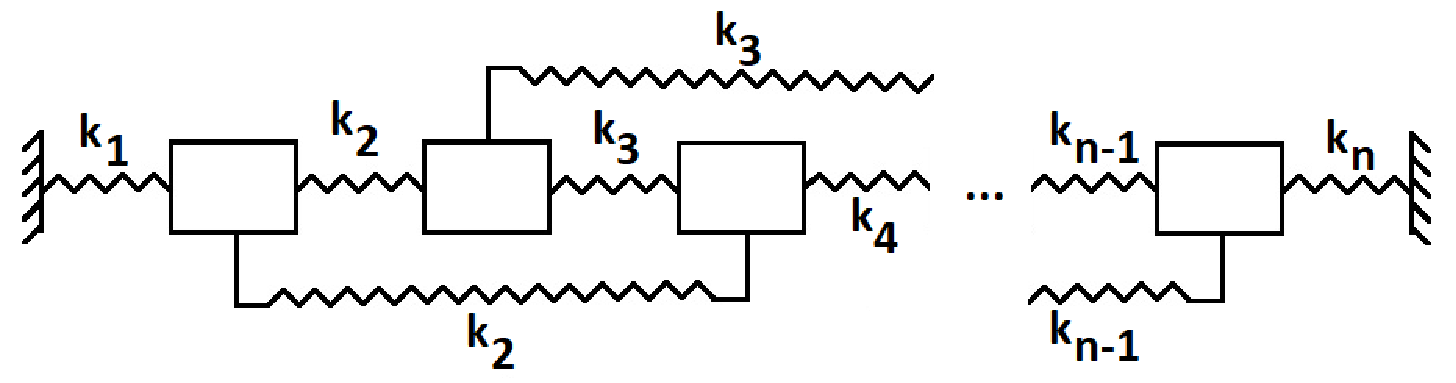
\includegraphics[width={3.0in}]{../figs/MassSys.pdf}
\centering
\caption{Equivalent spring-mass system used to generate the eigenvectors.}
\label{fig:stiff}
\end{figure}

Note that the values chosen do not need to represent physical systems (e.g. negative stiffness values are acceptable).  Thus, systems with positive, negative, and a combination of both were explored.  Two options were considered in coupling the masses with springs.  First, springs were added to couple the neighboring masses on the right and left.  
Both wall and cyclically symmetric (the last mass is coupled to the first) boundary conditions were tested.  The second type coupled the two neighboring masses on the left and right, while
applying wall boundary conditions.
As an example, Fig.~\ref{fig:stiff} shows the spring-mass system with springs connecting two neighboring masses and wall boundary conditions
that is further discussed in Section~\ref{sec:Eval}.  For brevity, the other coupling systems are not shown as the results were found to be not optimal.

Once the system is constructed, an eigenvalue problem is solved resulting in $n$ orthonormal eigenvectors used to represent the geometry for initial position $\theta=0$ and all initial $\phi$ positions.  
As the first vector tends to be planar motion (a cyclical vector) it is not chosen.  
This elimination results in a matrix formed by eigenvectors $2...m+1$.  
However, observations led to the conclusion that the orthogonal linear independence for $\theta=0$ caused some high $M$ values when considering all initial $\theta$ positions.  
Introducing linear dependence to the $\theta=0$ matrix was seen to result in decreased $M$ values for $\theta\neq 0$ combinations.  
To introduce linear dependence, a modified Gram-Schmidt orthogonality approach is used.  Specifically, 

\begin{equation}
\mathbf{E}^{new}_{d}=\mathbf{E}_{d}- c \sum_{e=1,...,n-1} \frac{\mathbf{E}_{e,e}^T \mathbf{E}_{d}}{\mathbf{E}_{e,e}^T \mathbf{E}_{e,e}}\mathbf{E}_{e,e},
\label{eq:GS}
\end{equation}

\noindent where $d$ denotes the $d^{th}$ eigenvector, $c$ is a constant between 0 and 1 such that 0 adds no linear dependence and 1 adds a portion of all other $\mathbf{E}_{e,e}$ vectors, and $e=1...n-1$ is the $e^{th}$ left shift of eigenvector $\mathbf{E}_e$. 
Thus, the similar component of shifted versions of each other vector, $\mathbf{E}_{e,e}$, is subtracted from the initially linearly independent basis ($\theta=0$) vectors. 

This formulation leads to a decrease in the $M$ values, but an increase in the individual MAC values for the basis vectors as the non-shifted vectors are no longer orthogonal.
Other combinations of eigenvectors and shifts for $\mathbf{E}_{e,e}$ are acceptable, however a shift is required due to the initial orthogonality (otherwise there is no similar portion to subtract).

Next, the average of each new eigenvector is subtracted from the corresponding vector. 
Since mask material may only be added, the minimum value (plus the 0.1 cm addition to the geometry) is added to the eigenvector to make all the thicknesses positive.  
Lastly, each eigenvector is normalized by the maximum vector value and scaled. 
These steps produce a minimal thickness of approximately 0.1 cm and a maximum mask thickness of 20 cm.

Multiple geometries for various $k$ and $c$ combinations can be tested resulting in the design surface shown in Fig.~\ref{fig:surf}.  
These results are based solely on the geometry vectors and not $\mathbf{DRM}_{red}$.  
Using this information, the $k$ and $c$ combination with the lowest $M$ value can be chosen for the more time expensive MCNP simulations.

\begin{figure}[ht!]
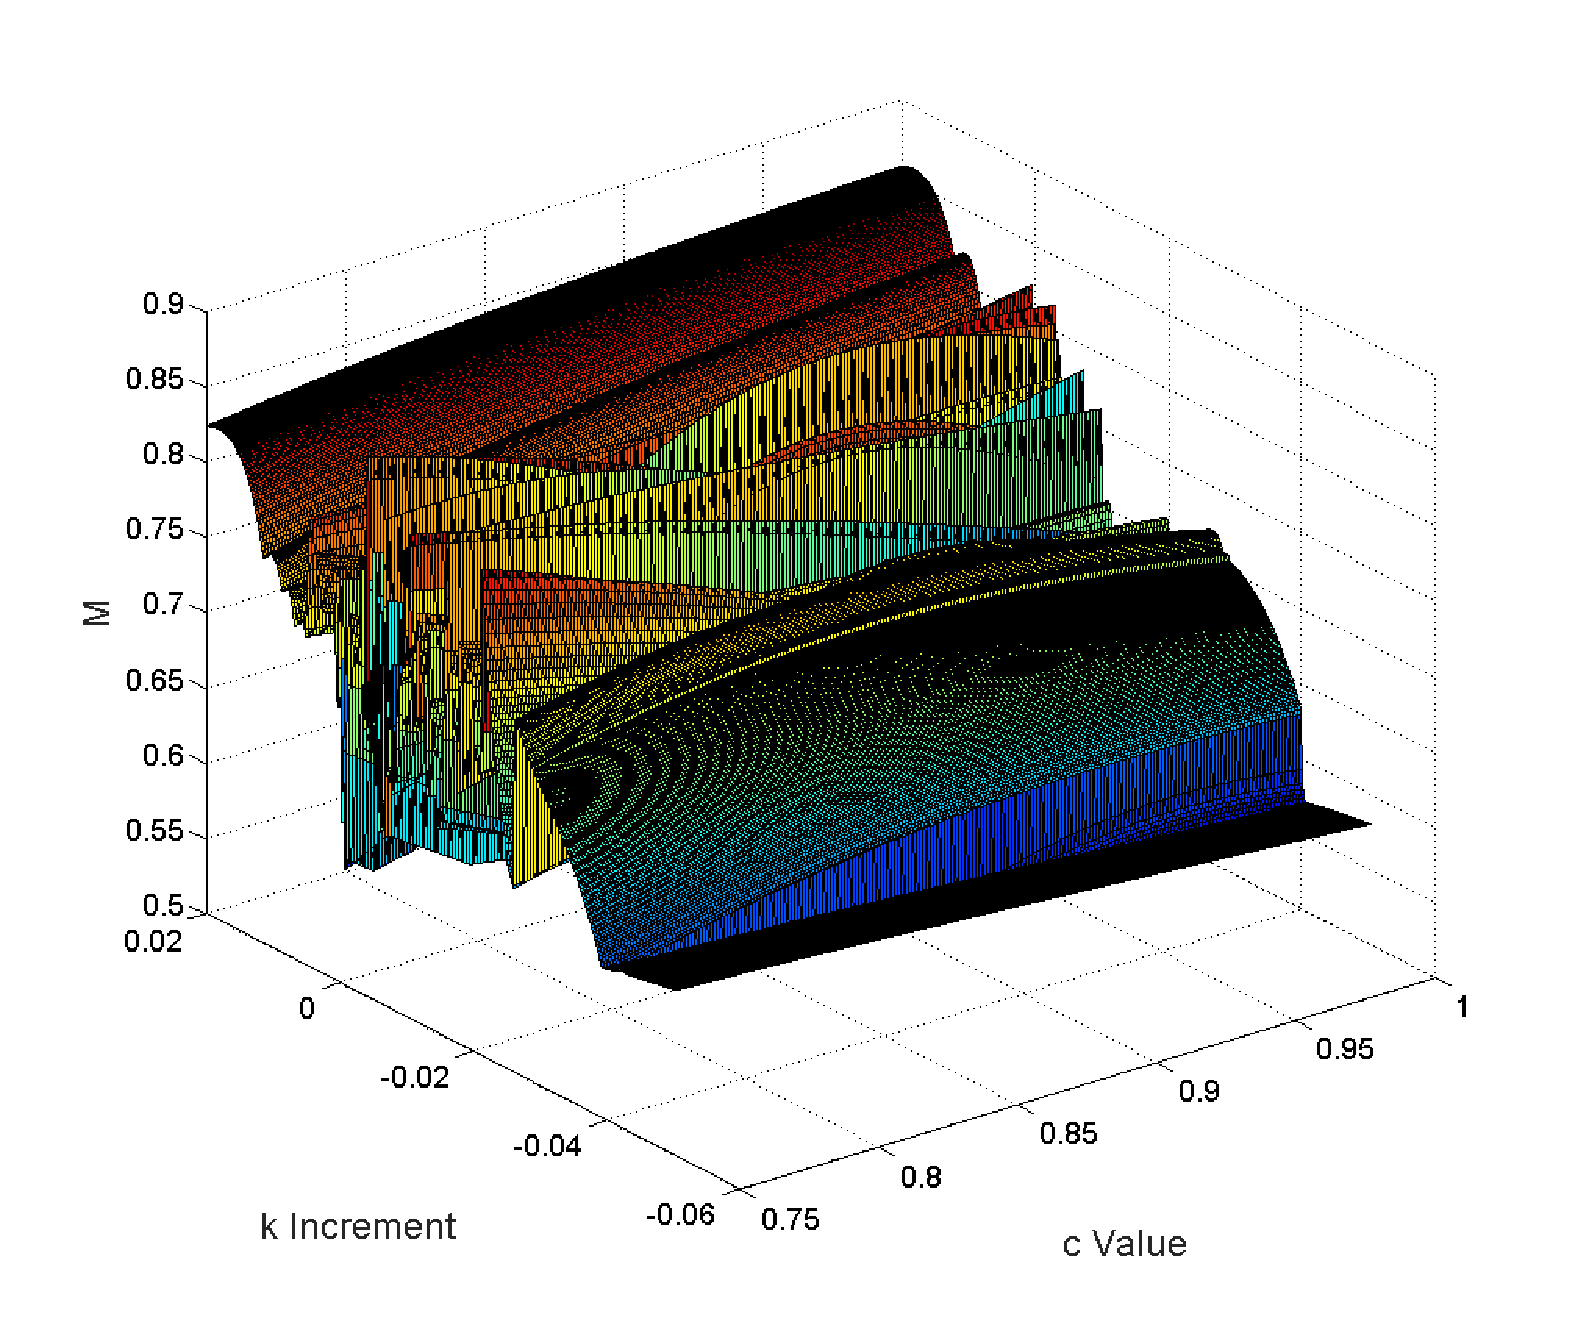
\includegraphics[width={3.0in}]{../figs/Eigprob32bitCouple2W1.pdf}
\centering
\caption{Design surface generated by different $k$ step increments and $c$ values used to minimize M.}
\label{fig:surf}
\end{figure}

\subsubsection{Binary Approach} \label{sec:binary}
The binary approach uses ones and zeros to represent the geometry thickness.  
Notice that the mask's cyclic nature causes vectors such as [1 1 0 0] to be the same as [1 0 0 1], where the first vector is the second shifted by one entry to the right.  
If the design uses binary patterns such as these two, the DRCs for two initial positions will be identical.  
As shown in \ref{sec:proof}, for $n>7$ any combination of vectors with three ones placed in an arrangement that avoids cyclic behavior with themselves (such as [1 0 1 0 1 0]) or others (such as [1 1 1 0 0 0] and [0 1 1 1 0 0]) produces a theoretical $M$ value of $4/9$.  
Note that including the binary ``1" vector represented using 6 bits as [0 0 0 0 0 1]) does not change this $M$ value.   
For $n=32$, there are many possible basis vectors; especially considering that the vectors can be shifted left or right (corresponding to multiplication or division by 2), and the $\phi$ vector order (1st, 2nd, 3rd, etc) may be swapped.  
This flexibility allows one to create unique geometries, mechanically balance the mask, or improve the likelihood of obtaining a signal given a random source position by more evenly spreading the ones and zeros around the mask.

\subsubsection{Decoupling $\theta$ and $\phi$}
\label{sec:decoupling}
An alternative approach introduces additional material to create a low measurement ``dead" zone at a consistent $\theta$ position.  
As a result, the initial $\theta$ position is assumed to be the angular distance difference between the start of the measurement and the minimum measurement location.  
The sign of the angle depends on the mask's rotation direction.  
It is conjectured that this association will be valid except when there are multiple sources in which spectral stripping is not possible or for distributed sources.  
Further work in this area is ongoing.

As the initial $\theta$ position is known, the reference DRM angle may be changed to the known $\theta$ position by shifting the basis matrix entries by the corresponding index number.
This knowledge decouples the $\theta$ and $\phi$ identification, resulting in only needing to compare the measured DRC to the $m$ $\phi$ curves in $\mathbf{DRM}_{red}$.  
Using this method, it is possible to create $m$ linearly independent geometric basis vectors.

One such linearly independent basis is the Hadamard matrix, which has been used in the design of stationary encoding masks in the fields of spectrometry and imaging \cite{Sloane76, Dyer91, Finger85}. 
What began as a one dimensional approach was extended to multi-dimensional problems \cite{Hammaker95, Hanley00, DeVerse00}, resulting in methods applicable to the RSM design optimization.
Of particular interest is Bellamy et al.'s attempt to produce a two dimensional, moveable encoding mask \cite{Bellamy97}.  Unfortunately, difficulties with mask positioning reproducibility and slow translation 
limit using moving mechanical masks in spectroscopy and imaging applications \cite{DeVerse00}.
Similar to the RSM design, Fateley et al. \cite{Fateley02} introduced a variable mask with a single element detector for spectroscopy and imaging use.  

While this matrix has been used in spectroscopy for many years, Hadamard encoding masks assume that some of cells are ``on", ``off", or detected by a second sensor \cite{DeVerse00}.  
In addition, it is assumed that one knows the on/off state of the cells.  
The equivalent RSM design goal is to identify this on/off state and thus, it corresponds to an inverse problem.  
In contrast to the encoding masks, each cell in the RSM design is not in a fully on/off state, but may have particles passing through it even when the source is not directly aligned.

The Hadamard matrix is thought to only exist for square matrices where $n$ is 1, 2, or divisible by 4 \cite{Sloane76}.  
By construction, the mask design under consideration is discretized in order to have $n=32$.  
Also, a Hadamard matrix has ones and negative ones.  
To convert it to a binary pattern, the negative one entries were changed to zeros.
In order to create the "dead" zone, the vector of ones corresponding to $\theta=0$ were changed to twos.  
A normalized geometry resulted by following the same steps as outlined in the eigenvector approach.

\subsection{Design Evaluation}
\label{sec:Eval}
To assess the design optimality, four criteria relevant to the performance of the RSM are proposed.  The first, the maximum MAC value, was discussed in Section~\ref{sec:MAC}.  
The average MAC number, $A$, is given in Eqn.~\ref{eq:avgmac} and provides information about the mean linear dependence.
\begin{equation}
A=\frac{1}{b}\sum_{g,h,i,j}\left(MAC_{g,h,i,j}\right),
\label{eq:avgmac}
\end{equation}

\noindent where $g\neq i$, $h\neq j$, and $b$ is the total number of combinations given by $b=\left(\overset{m}{_2}\right)+(n-1)\left(\overset{m+1}{_2}\right)$.  
Note that $\left(\overset{m}{_2}\right)$ is the total number of combinations without $\theta$ shifts (aka $\theta=0$), $n-1$ is the total number of $\theta$ shifts possible, and $\left(\overset{m+1}{_2}\right)$ is the number of combinations for DRCs shifted one $\theta$ position.  
For the $n=32$ and $m=30$ mask design, $b=14850$.  The optimal design should have low $M$ and $A$ values.

The average, minimum, and maximum DRC values for a given $\phi$ remain the same for different initial $\theta$ values.  
Thus, no $\theta$ shifting needs to be considered in the following two criteria.  The third criteria measures the RSM's average efficiency for a mask cell. 
A high-efficiency design produces more accurate results in less measurement time, an important factor to consider for the intended RSM applications.  
This value is calculated as 

\begin{equation}
\epsilon=\frac{\sum_{i,j}\mathbf{DRM}_{red}}{n\ m},
\label{eq:avgcell}
\end{equation}

\noindent where $n\ m$ is the total number of mask cells.
Note, this is not the absolute detection efficiency as the spectra obtained remove the $<$ 200~keV counts.

The final evaluation criterion focuses on the design's sensitivity.  
The ratio of the maximum to minimum response in Eqn.~\ref{eq:sens} provides information on the relative amount of measurement time required and the measurement's sensitivity to random measurement noise. 

\begin{equation}
S=min_{j}\left(\frac{max_{i} \left[\mathbf{DRM}_{red}\right]}{min_{i} \left[\mathbf{DRM}_{red}\right]}\right).
\label{eq:sens}
\end{equation}

The following section applies the four evaluation criteria to DRC simulations for all possible discrete source positions for the designs generated from the three approaches outlined in Sec.~\ref{design-methods}.

\section{Results and Analysis} \label{sec:results}
The proposed design methodologies produced the geometries shown in Figs.~\ref{fig:EVGeo} to \ref{fig:HadGeo}.

\begin{figure}[ht!]
\centering
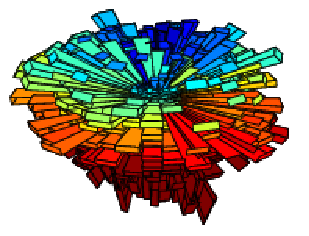
\includegraphics[width={2.0in}]{../figs/EVGeo.pdf}
\caption{RSM geometry created by the eigenvector approach.}
\label{fig:EVGeo}
\end{figure}

\begin{figure}[ht!]
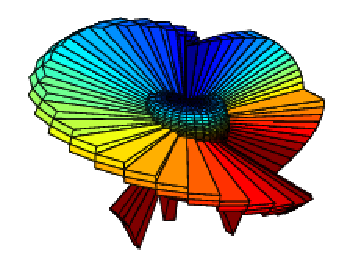
\includegraphics[width={2.0in}]{../figs/BiGeo.pdf}
\centering
\caption{RSM geometry created by the binary approach.}
\label{fig:BiGeo}

\end{figure}
\begin{figure}[ht!]
\centering
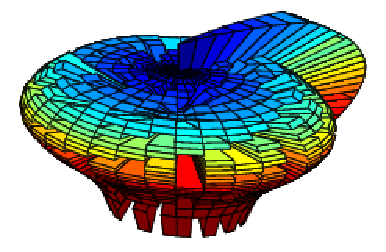
\includegraphics[width={2.0in}]{../figs/HadGeo.pdf}
\caption{RSM geometry created by the Hadamard approach.}
\label{fig:HadGeo}
\end{figure}

The eigenvector approach used 32 $k$ values from 0.1 to -0.2999 in increments of -0.0129 with stiffness coupling to the nearest two neighbors on both sides of the mass.
$c$ was determined to be 0.999 from the design surface minimization depicted in Fig~\ref{fig:surf}.  
Other coupled systems did not have an optimal $c$ value close to one.

The binary pattern was constructed to have a fin that spirals around the mask.  
As it is not possible to have the fin completely cover the mask geometry, four other vectors were added to create the necessary basis.

The FitzGerald's RSM was used as a baseline to establish the design improvement for the RSM designs shown in Figs.~\ref{fig:EVGeo} to \ref{fig:HadGeo}.  
The simulation of FitzGerald's design involved a mask discretization of 10$^\circ$ in $\theta$ and $\phi$; corresponding to $n=36$.  However, the Hadamard $n=36$ matrix cannot be created by lower order Hadamard matrices \cite{Weisstein}, thus the proposed designs use $n=32$. 
This change in discretization will only have a minor impact to the evaluation criteria as the discretizations are sufficiently coarse to avoid the spatial resolution limit for a single point source.

Figure~\ref{fig:RSMMAC} shows a visual MAC number representation for $\theta=0$ obtained by using Eqn.~\ref{eq:mac}. 
 
\begin{figure}[ht!]
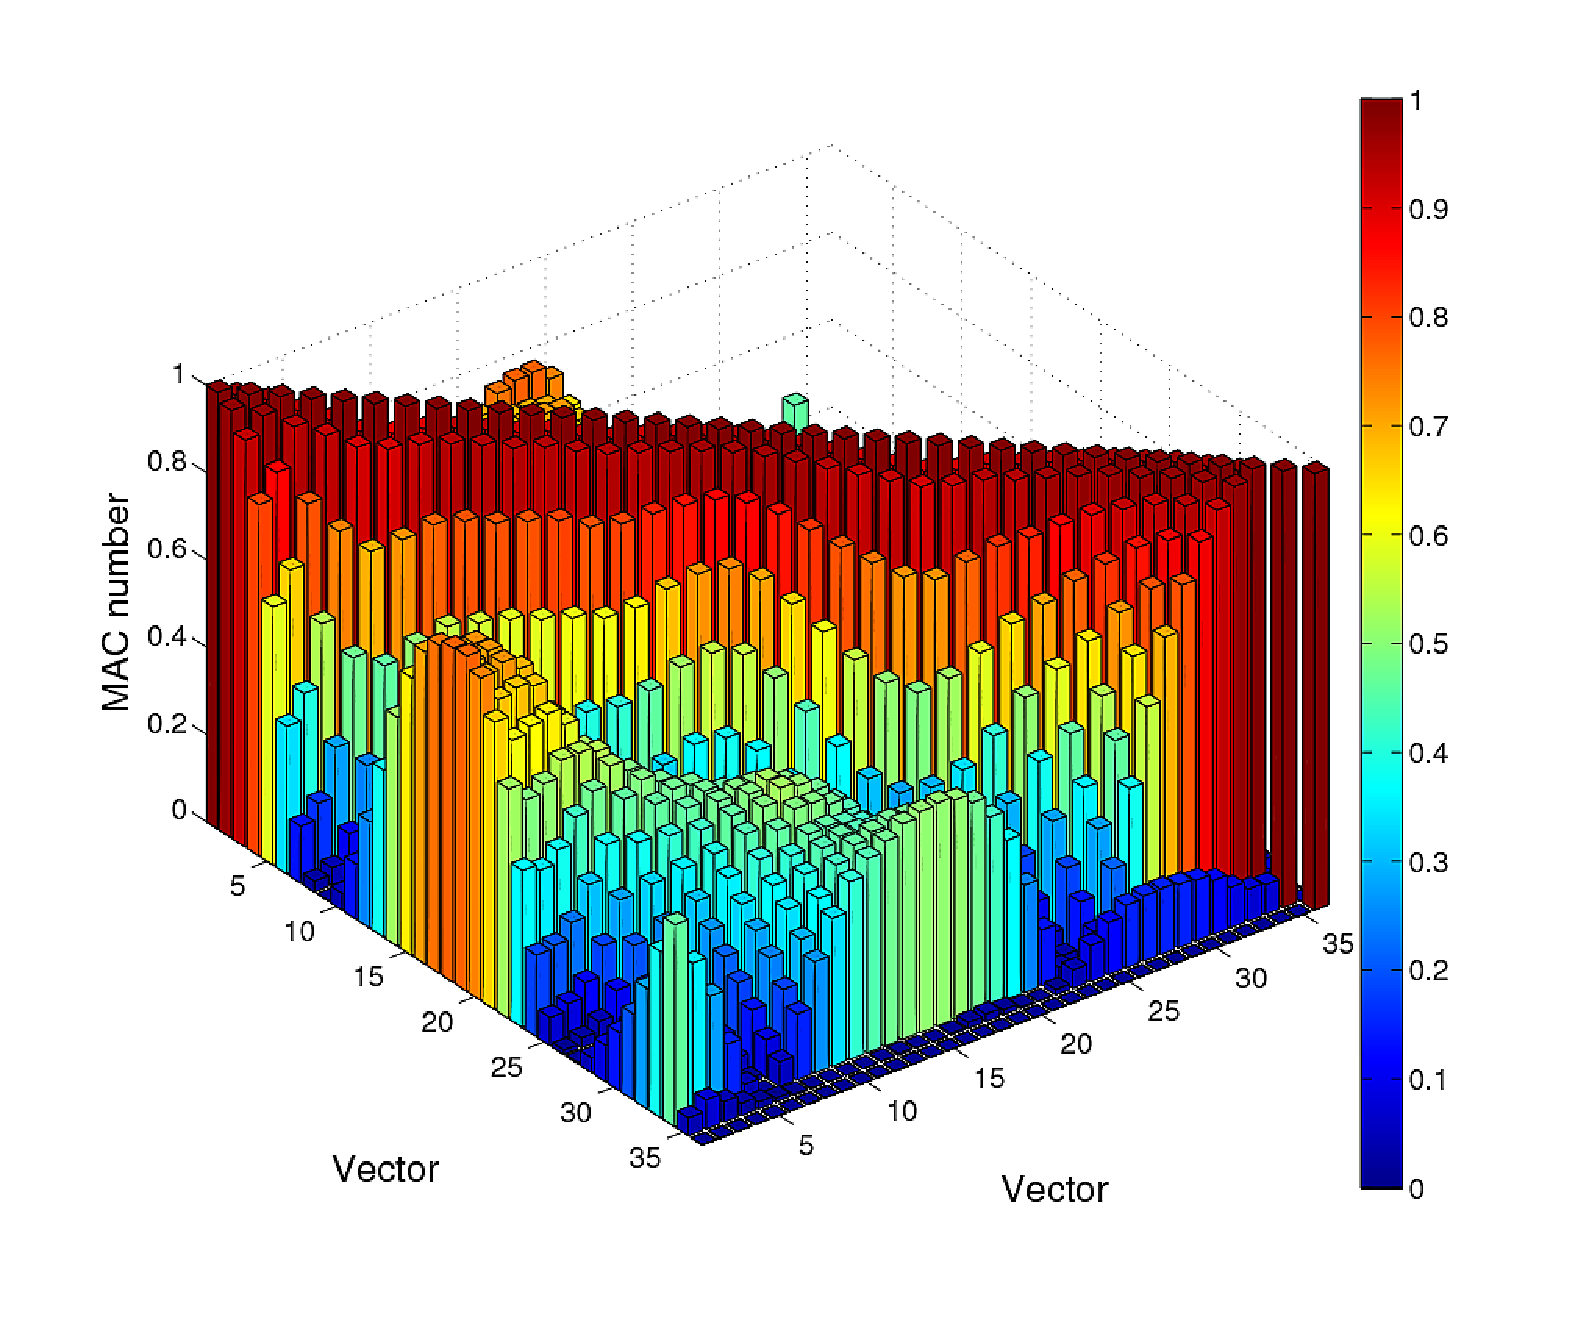
\includegraphics[width={3.0in}]{../figs/RSMMAC.pdf}
\centering
\caption{Representation of the Fitzgerald RSM MAC numbers for $\theta=0$.}
\label{fig:RSMMAC}
\end{figure}

It is worth pointing out a couple of key features for these MAC plots. 
First, the diagonal entries correspond to comparing a vector to itself, and thus will always be equal to one.
Second, the plots are symmetric about the diagonal.  
Finally, the large off-diagonal regions are of particular interest because these high values could result in the mis-identification of the source direction. 
The new proposed designs significantly lower off-diagonal values resulting in less degeneracy in the source direction as shown in Figs.~\ref{fig:EMAC} to \ref{fig:HadMAC}.

\begin{figure}[ht!]
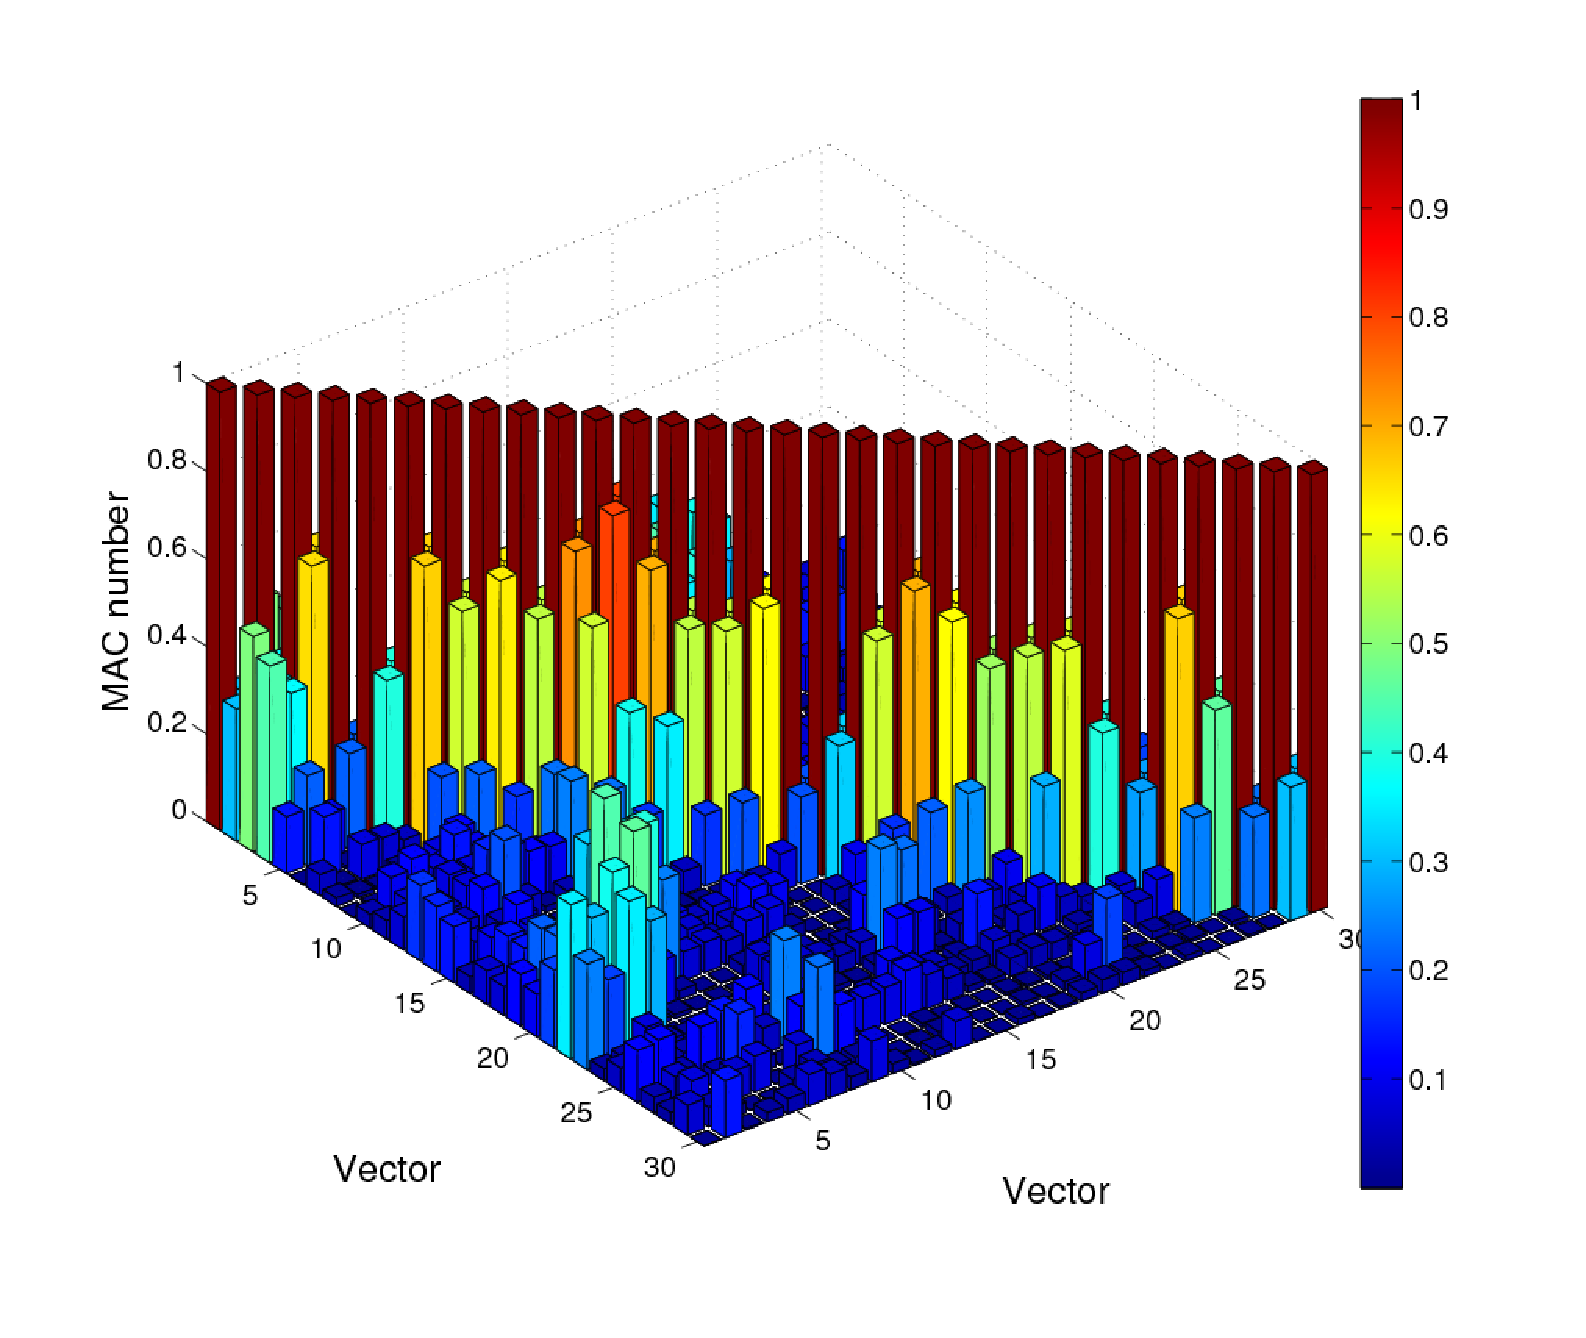
\includegraphics[width={3.0in}]{../figs/EVMAC.pdf}
\centering
\caption{Eigenvector RSM MAC values for the basis $\theta=0$.}
\label{fig:EMAC}
\end{figure}

\begin{figure}[ht!]
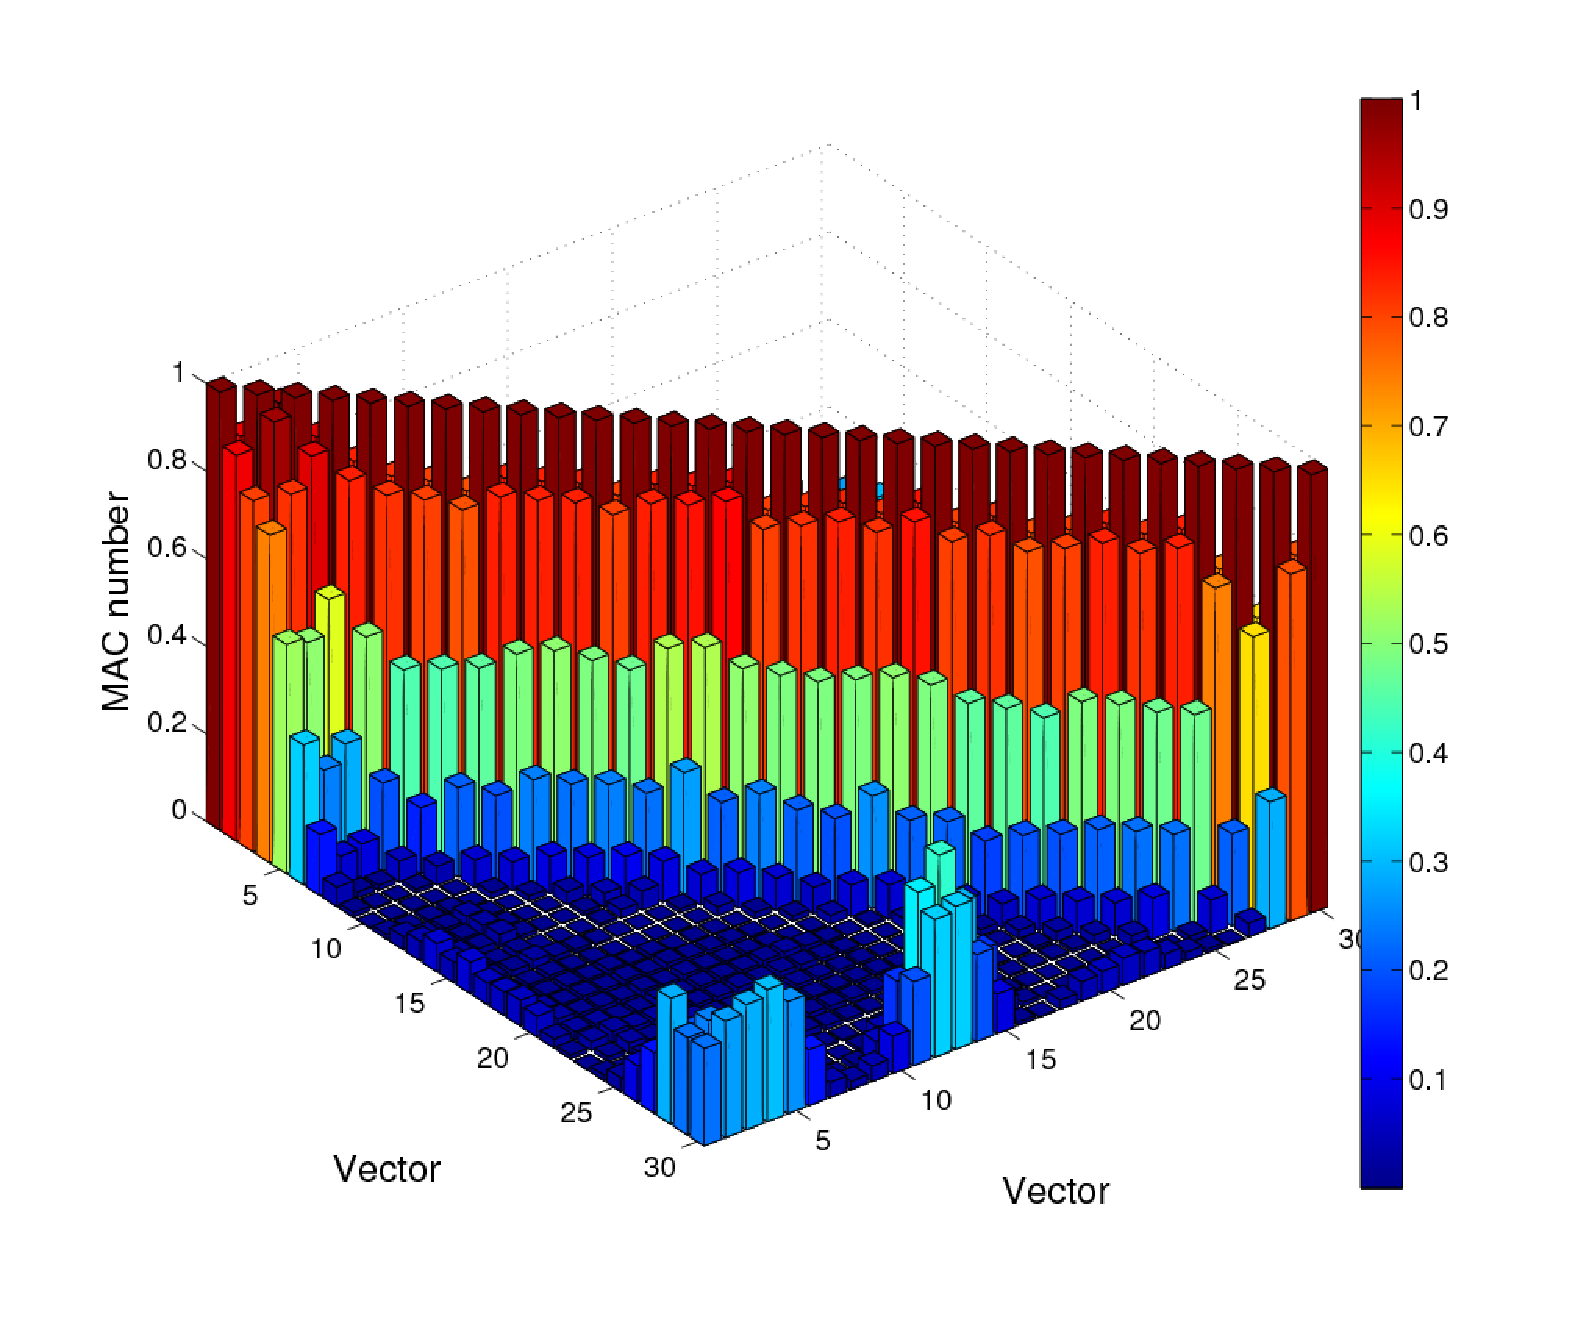
\includegraphics[width={3.0in}]{../figs/BiMAC.pdf}
\centering
\caption{Binary RSM MAC values for the basis $\theta=0$.}
\label{fig:BMAC}
\end{figure}

\begin{figure}[ht!]
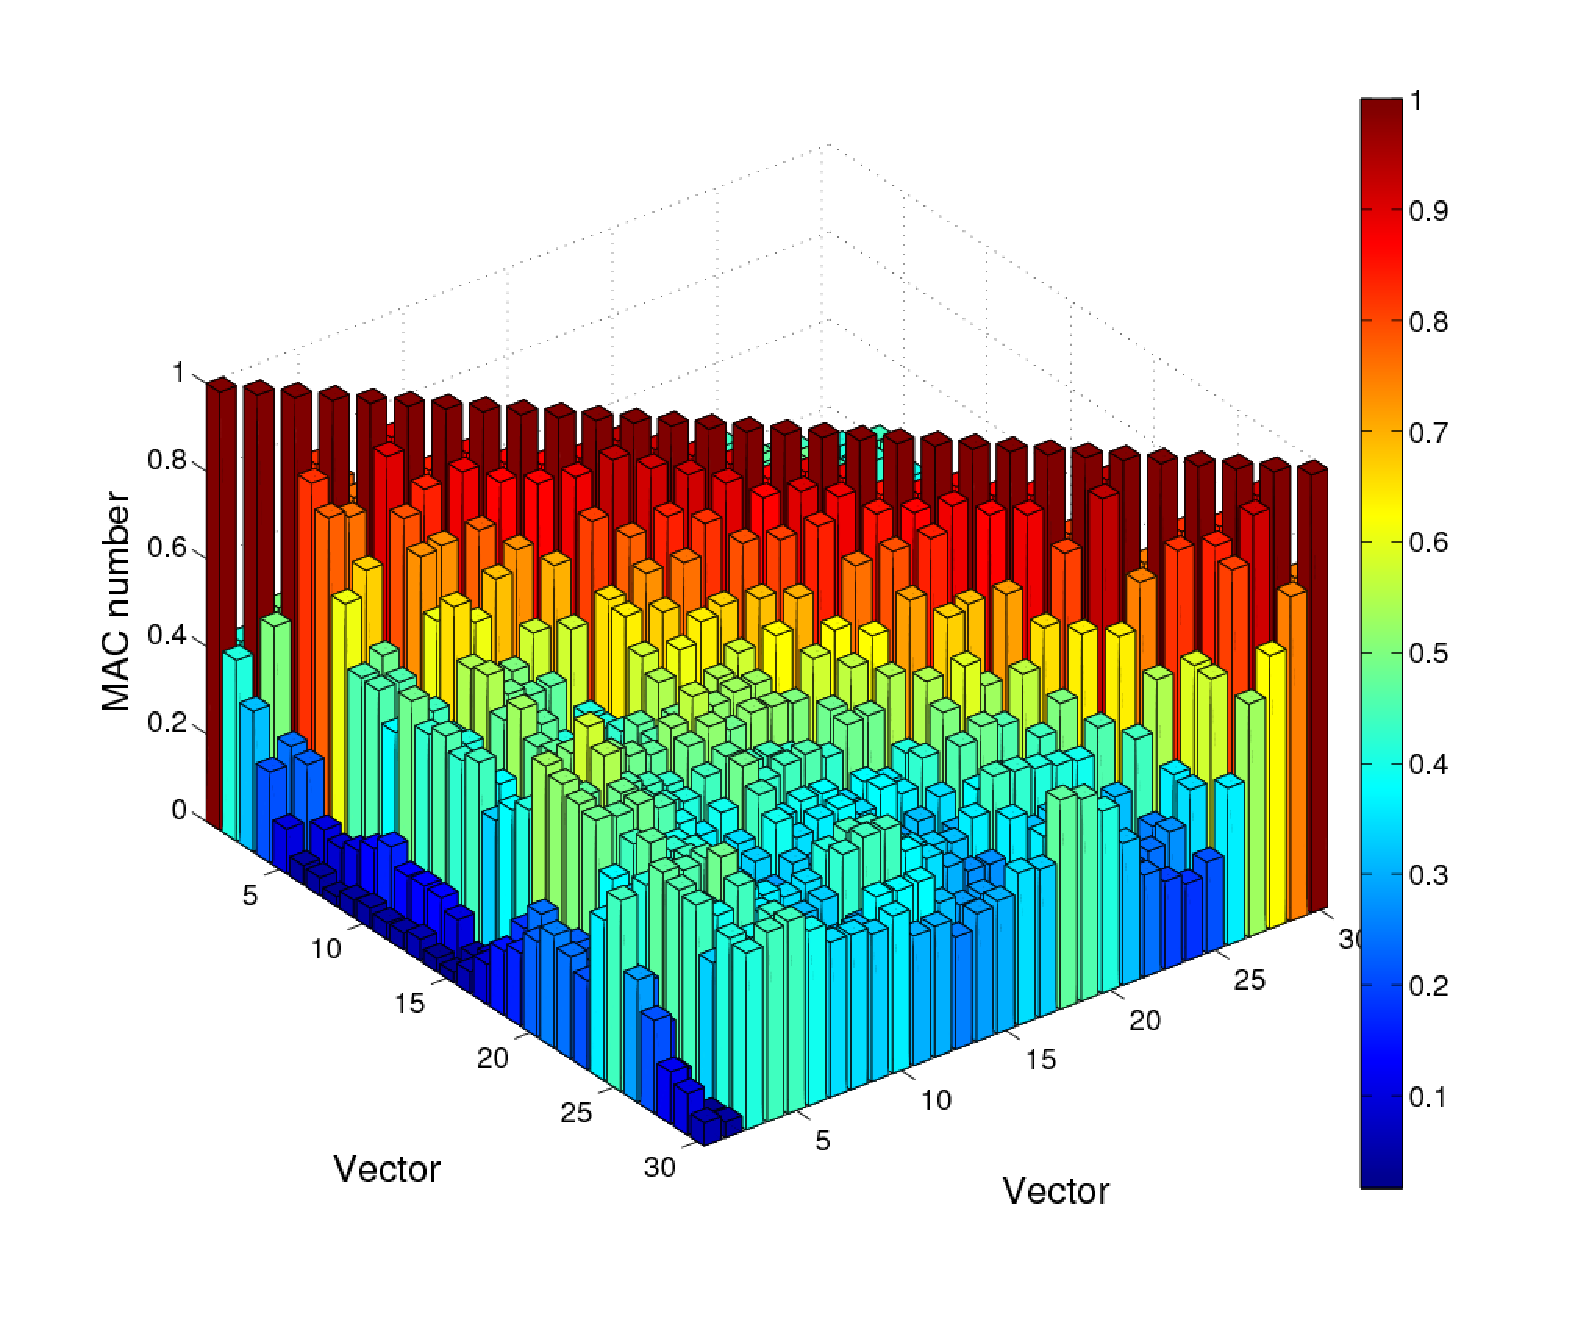
\includegraphics[width={3.0in}]{../figs/HadMAC.pdf}
\centering
\caption{Hadamard MAC numbers for the basis $\theta=0$.}
\label{fig:HadMAC}
\end{figure}

The adjacent off-diagonal terms in Figs.~\ref{fig:RSMMAC}, \ref{fig:BMAC}, and ~\ref{fig:HadMAC} show that there is a limit to the spatial resolution.  
Specifically, vectors $j$, $j+1$, $j+2$, and $j+3$ have MAC numbers that incrementally decrease indicating that information is shared by neighboring initial positions.  
In the presence of measurement noise, it may only be possible to identity the position to an accuracy that is a multiple of the $\theta$ or $\phi$ discretization.

The off diagonal terms for the binary design are indicative of the limits of the design approach pursued.  
Since a full optimization was not performed, it is likely that the binary design can be improved by replacing the last four vectors with alternatives. 
This could result in a decrease in the off-diagonal terms corresponding to these four vectors thereby improving the performance characteristics of this design class.

Table~\ref{table:results} summarizes the evaluation results for the original RSM, binary, eigenvector (EV), and Hadamard approaches.  
Recall that the Hadamard values correspond to those obtained without shifting vectors since the initial $\theta$ position can be deduced.

\begin{table}[ht]
\caption{Evaluation criteria comparisons from the original design and the three proposed designs from this work.} % title of Table
\centering % used for centering table
\begin{tabular}{|c|c|c|c|c|} % centered columns (4 columns)
\hline
Criteria & Fitzgerald & EV & Binary & Hadamard\\
\hline
M & 1.00 & 0.808 & 0.963 & 0.935\\
\hline
A & 0.210 & 0.0663 & 0.125 & 0.423 \\
\hline
$\epsilon \left(\times 10^{-4}\right)$ & 3.75 & 2.96 & 3.86 & 3.70\\
\hline
S & 1.00 & 1.07 & 1.16 & 1.07 \\
\hline
\end{tabular}
\label{table:results} % is used to refer this table in the text
\end{table}

Notice that the original design has a maximum MAC number of 1.00. 
This value corresponds to a part of the geometry that has a constant thickness as $\theta$ varies.  
As a result, a shift in the initial $\theta$ produces the same DRC and a MAC number of 1.  
For the same reason, the sensitivity value is 1.00.  
In contrast, the proposed methods have lower $M$ values with the most desirable corresponding to the eigenvector approach.  
The Hadamard method produces vectors which on average share 42.3\% of their information, which is more than the original design.  
The rapid change between ones and zeros coupled with the spatial resolution limits make the Hadamard method non-ideal for this problem.  
The lowest average MAC number corresponds to the eigenvector approach with only 6.63\% similarity.  
These results indicate that the method that produces the most unique
DRCs is the eigenvector approach.  
However, the trade-off is that the eigenvector method produced a RSM with a lower average normalized number of counts per cell.  
The binary method has the most average normalized number of counts per cell, but also the highest sensitivity.  
This high sensitivity may indicate that certain initial positions are more susceptible to measurement noise.


\section{Conclusions} \label{sec:conclusions}
Rotating scattering masks (RSMs) have shown promise for a gamma source direction identification, 
but previous results indicate that the original RSM design has degenerate detector response curves.  
This degeneracy may result in an incorrect source position identification, especially when considering noise, finite count times, and statistical confidence intervals.
To improve upon the current state-of-the-art, this work introduced three methods to optimize the RSM geometry to limit the mis-identification of a gamma source's direction.  

The eigenvector approach produced the most unique detector response curves when compared to the original Fitzgerald RSM and other proposed methodologies. 
Thus, this approach reduces the source direction mis-identification possibility inherent to the Fitzgerald design.
Unfortunately there is a corresponding decrease in the average normalized counts per cell.
On average the eigenvector mask requires 21\% more particles and, therefore, longer measurement times to produce the same statistical accuracy as the original design.
However, due to an increase in DRC differentiation for initial positions exhibiting a high off-diagonal maximum MAC, the count number needed to correctly identify these source directions will increase by less than 21\% and may decrease. 

While these results demonstrate the binary and eigenvector methods decrease the overall and average linear dependence of the DRCs, the full design space was not explored and more optimal designs may exist.  
Specifically, choosing an alternative last four vectors for the binary pattern may reduce the corresponding off-diagonal MAC terms, and, as a result, $A$ should decrease.  
Additionally, rotating or swapping the binary vectors would allow for a better mechanical balance.  
Finally, the eigenvector approach has a large design space especially when other coupled systems are considered.  
Further exploration of this space and its refinement may produce a geometry with lower $M$ and $A$ values.

\section{Acknowledgment}
This work was supported though the Air Force Summer Faculty Program and the Air Force Institute of Technology.  
The authors would to thank Dr. Ashley Holland and Dr. Adam Cahill for their assistance and insightful input to this work.

\appendix

% This is not referenced at all in the paper.
% Added to binary approach section
\section{Binary Approach Proof} \label{sec:proof}
The objective of the following work is to choose $n$ binary numbers such that the MAC number denoted as 

\begin{equation}
MAC_{a,b}=\frac{\left(\mathbf{a}\cdot\mathbf{b}\right)^2}{\left(\mathbf{a}\cdot\mathbf{a}\right)\left(\mathbf{b}\cdot\mathbf{b}\right)}
\end{equation}

\noindent is minimized for every combination of numbers $\textbf{a}$ and $\textbf{b}$ including their the corresponding cyclically shifted versions.

Consider an $n$ bit binary number greater than zero with $p$ ones and $n-p$ zeros, where $0<p<n$.  
Further, shift this number by a number of bits so that the left-most bit contains a one.  
Because of the mask's cyclic nature, the binary number can be written as a vector containing the integer number of zeros bounded on either end by ones.  
For example, the number 0 1 1 would be shifted to 1 0 1 and could be written as the vector [1].  
Also, the number [0 1 0 1 0 1 0 0] can be shifted to [1 0 1 0 1 0 0 0], and the corresponding vector is [1 1 3].  
Recall that the vector's cyclic nature causes the last one to wrap around to the first 
position.  
In general, we can write any non-zero binary number as the vector $\textbf{v}=\left[v_1\ v_2\ v_3\ \cdots\ v_p\right]$, where each $v_i$ is the number of zeros between two ones and $v_p=n-p-\sum\limits_{i} v_i$.  

Now, cyclic redundancy can be avoided by ignoring any $\textbf{v}$ that become duplicated under shifts.  
For example, [0 3 2] and [3 2 0] represented the same binary number, where the second vector is the first shifted to the left by $v_1+2$ bits.  
To avoid this behavior, we require $v_{1}<v_p$ and $v_2\le v_p, v_3\le v_p, \cdots, v_{p-1}\le v_p$.  
Note that by construction two vectors with a different number of ones cannot be cyclically identical.

Consider two vectors, $\textbf{u}=\left[u_1\ u_2\ u_3\ \cdots\ u_{p_u}\right]$ and $\textbf{v}=\left[v_1\ v_2\ v_3\ \cdots\ v_{p_v}\right]$ containing $p_u$ and $p_v$ ones respectively.  
If $u_i=v_i$ the vector has at least two ones in the corresponding binary number that would align for some shift of $\textbf{u}$.  
We want to choose $n$ vectors, $a_1, a_2, ... a_n$, that produce the minimum value of $max\left\{MAC_{a_1...a_n}\right\}$, where the maximum is taken over all possible shifts of $\textbf{a}_i, \textbf{a}_j$, $i=1...n$, and $j=1...n$.  
Note that if $i=j$, then the second vector must be shifted by at least one bit to avoid comparing a vector with itself.  
For a binary number undergoing all possible shifts, the denominator becomes $p_u p_v$, while the numerator is the square of the total number of ones that simultaneously align as each vector is rotated.  
As the number of ones increases, denominator increases, while the numerator remains the same or increases.   
Thus, it becomes unclear if the MAC number increases or decreases as $p_u$ and/or $p_v$ increase.

First, consider $p=1$.  There is only one non-cyclically redundant vector, which can be expressed as $\left[n-1\right]$.  
Letting $\textbf{a}$ be this vector and $\textbf{b}$ be any shifted version of the vector results in a maximum MAC number of $\frac{0}{1*1}=0$.

Next, consider $p=2$.  Recall that a $p=2$ type vector contains two 1s, so if two 1s aligned the vectors would be identical.  
By construction, all of the possible $p=2$ indices should be unique indicating that only one 1 aligns over all possible rotations.
Thus, possible non-redundant vectors include $[0\ n-p], [1\  n-p-1], [2\ n-p-2], \cdots, [\frac{n-p-1}{2}\ \frac{n-p+1}{2}]$ if $n$ is odd or a limit of $[\frac{n-p}{2}-1\ \frac{n-p}{2}+1]$ if $n$ is even.    
Also, there are only $\frac{n-p+1}{2}$ (if $n$ is odd) or $\frac{n-p}{2}$ (if $n$ is even) possible $p=2$ type vectors, but $n$ are desired.  
Thus, more vectors from other $p$ types would be required to complete the $n$ basis set.    
As a result, the maximum MAC number for any two $p=2$ vectors is $\frac{1^2}{2*2}=1/4$.

Consider $p=3$, the set of all binary vectors containing three 1s.  
Let the matrix $\textbf{V}$ contain terms $V_{ij}=v_i$ for the $j^{th}$ basis vector including the dependent $v_p$, where $1<i<p$ and $1<j<n$.
For a given $n$ and $p$, the number of unique indices is less than or equal to $\lfloor \frac{n-p}{2}\rfloor+1$ since $v_i\le v_p$.  
Any column in $\textbf{V}$ contains $n$ values.  Thus, it is not possible for one column to only contain unique indices since $n>\lfloor \frac{n-p}{2}\rfloor+1$.
This result implies that it is impossible to form a complete basis using only $p=2$ type vectors as previously mentioned.  In addition, a $p=3$ basis must have
duplicate indices.

However, it is possible to create an $n$ basis, where only one index in each $p=3$ vector is duplicated over all vector shift considerations.  
This $p=3$ basis has a maximum MAC number equal to $\frac{2^2}{3*3}=4/9$, where one duplicate index results in two aligned 1s.
Let $q=\lfloor\frac{n-p-1}{p}\rfloor$, $r=\lfloor\frac{n-p}{2}\rfloor$, and $s$ is 0 if $n$ is odd and 1 if $n$ is even, where $\lfloor\ \rfloor$ denotes the floor function.
Possible vectors with $v_1\le q$ form sets of decreasing size

\begin{center}
$\{[0,\ 0,\ n-p-0]; [0,\ 1,\ n-p-1]; \cdots [0,\ r-0,\ r+s-0]\}$,\\
$\{[1,\ 0,\ n-p-1]; [1,\ 1,\ n-p-2]; \cdots [1,\ r+s-1,\ r-0]\}$,\\
$\{[2,\ 0,\ n-p-2]; [2,\ 1,\ n-p-3]; \cdots [2,\ r-1,\ r+s-1]\}$,\\
$\{[3,\ 0,\ n-p-3]; [3,\ 1,\ n-p-4]; \cdots [3,\ r+s-2,\ r-1]\}$,\\
$\{[4,\ 0,\ n-p-4]; [4,\ 1,\ n-p-5]; \cdots [4,\ r-2,\ r+s-2]\}$,\\
$\vdots$ \\
$\{[q,\ 0,\ n-p-q], [q,\ 1,\ n-p-q-1], \cdots [q,\ r-\lfloor \frac{q+1}{2}\rfloor+s\ mod(q,2),\ r-\lfloor \frac{q}{2}\rfloor+s\ mod(q+1,2)]\}$.
\end{center}

In general, the $i^{th}$ set ($i=0\ ...\ q$) can be expressed as 

\begin{equation}
\{[i,\ 0,\ n-p-i], [i,\ 1,\ n-p-i-1], \cdots [i,\ r-\lfloor \frac{i+1}{2}\rfloor+s\ mod(i,2),\ r-\lfloor \frac{i}{2}\rfloor+s\ mod(i+1,2)]\},
\end{equation}

\noindent where the total number of terms, $t_1$, is

\begin{equation}
t_1=\sum_{i=0}^{q} \lfloor\frac{n-p}{2}\rfloor-\lfloor\frac{i+1}{2}\rfloor+s\ mod(i,2)+1.
\end{equation}

\noindent Since $v_1<v_3$, sets with $v_1>q$, can be expressed using the following approach,

\begin{center}
$\{[q+1,\ 0,\ n-p-q-1]; [q+1,\ 1,\ n-p-q-2]; \cdots [q+1,\ n-p-2q-3,\ q+2]\}$,\\
$\{[q+2,\ 0,\ n-p-q-2]; [q+2,\ 1,\ n-p-q-3]; \cdots [q+2,\ n-p-2q-5,\ q+3]\}$,\\
$\{[q+3,\ 0,\ n-p-q-3]; [q+3,\ 1,\ n-p-q-4]; \cdots [q+3,\ n-p-2q-7,\ q+4]\}$,\\
$\vdots$ \\
\end{center}

\begin{center}
$\{[\lfloor\frac{n-p-1}{2}\rfloor,\ 0,\ r+1]\}$ if $n$ is even.\\
$\{[\lfloor\frac{n-p-1}{2}\rfloor,\ 0,\ r+1]; [\lfloor\frac{n-p-1}{2}\rfloor,\ 1,\ r]\}$ if $n$ is odd.
\end{center} 

\noindent In general, the $i^{th}$ set ($i=q+1\ ...\ \lfloor\frac{n-p-1}{2}\rfloor$) can be expressed as 

\begin{equation}
\{[i,\ 0,\ n-p-i-0], [i,\ 1,\ n-p-i-1], \cdots [i,\ n-p-2i-1,\ i+1]\},
\end{equation}

\noindent where the total number of terms, $t_2$, is

\begin{equation}
t_2=\sum_{i=q+1}^{\lfloor\frac{n-p-1}{2}\rfloor} n-p-2i-1+1 =\sum_{i=q+1}^{\lfloor\frac{n-p-1}{2}\rfloor} n-p-2i
\end{equation}

\noindent Thus, the total number of terms for $p=3$ and a given $n$ is $t=t_1+t_2$.  

Recall that $p=1$ only has a single ``1" which will align with any $p=3$ vector for three shifted positions.  
As a result, the $p=1$ vector can be combined with the $p=3$ vectors, since the maximum MAC number between a $p=1$ and $p=3$ vector is $\frac{1^2}{1*3}=\frac{1}{3} < \frac{4}{9}$.  
Figure~\ref{fig:terms} shows that the number of possible $p=3$ terms (including $p=1$) equals (if $n=8$) or exceeds $n$ (if $8<n\le 360$).  
Due to manufacturing constraints, $n$ was limited to 360 as this corresponds to one degree increments in $\theta$ and 0.5 degree in $\phi$.  
As a result, if $n>7$ a full $n$ basis with a $\frac{4}{9}$ maximum MAC number can be formed from these vectors.

\begin{figure}[ht!]
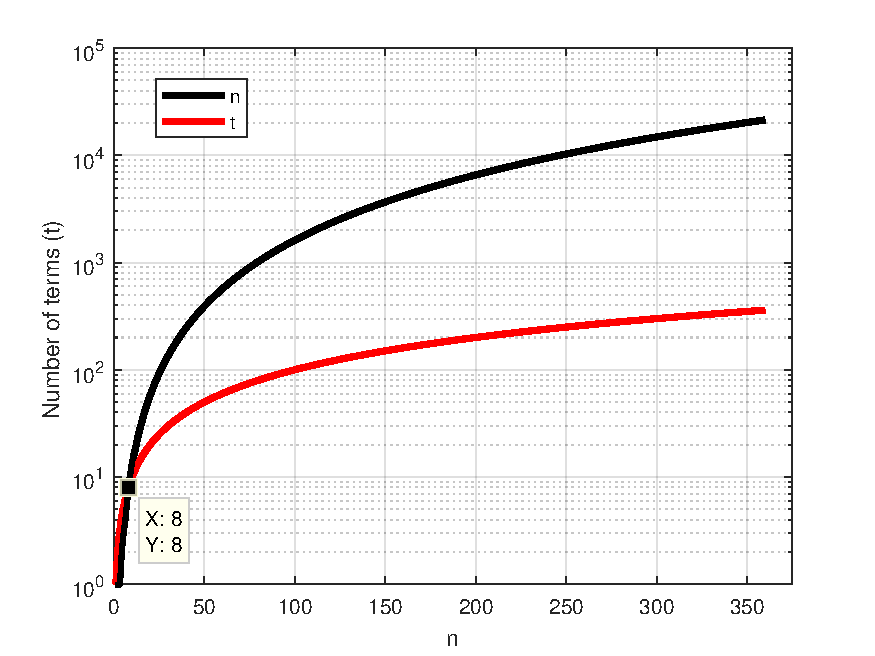
\includegraphics[width={3.0in}]{../figs/TermPlot.pdf}
\centering
\caption{The number of possible terms for $p=1$ and 3 equals or exceeds $n$ if $n>7$.}
\label{fig:terms}
\end{figure}

Now, consider creating a basis using both $p=2$ and $p=3$ vectors.  Since some of the vector indices are duplicated, there are three resulting cases.
First, if all the vectors with duplicate entries are of type $p=3$, then the maximum MAC number remains the previously derived $\frac{4}{9}$, $p=3$ value.  
Second, $p=2$ cannot have duplicated entries with other $p=2$ vectors as these vectors only have one degree of freedom.  The index duplication would
result in duplicated $p=2$ vectors and a maximum MAC number of $1$.  The previous $p=2$ construction addressed this issue.
Lastly, if a $p=2$ vector index matches a $p=3$ vector index, then the maximum MAC number is $\frac{2^2}{2*3}=\frac{2}{3}>\frac{4}{9}$.  
Combining $p=2$ and $p=3$ type vectors will not decrease the maximum MAC number and if done incorrectly, could increase its value
to $\frac{2}{3}$.

%% References
%%
%% Following citation commands can be used in the body text:
%% Usage of \cite is as follows:
%%   \cite{key}         ==>>  [#]
%%   \cite[chap. 2]{key} ==>> [#, chap. 2]
%%

%% References with BibTeX database:

\bibliographystyle{elsarticle-num}
\bibliography{RSM}

%% Authors are advised to use a BibTeX database file for their reference list.
%% The provided style file elsarticle-num.bst formats references in the required Procedia style

%% For references without a BibTeX database:

% \begin{thebibliography}{00}

%% \bibitem must have the following form:
%%   \bibitem{key}...
%%

% \bibitem{}

% \end{thebibliography}

\end{document}

%%
%% End of file `ecrc-template.tex'. 